\section{Introduction} \label{man-introduction}
This section will go in detail about the workings, idea's and logic of our expert system.

\section{Application} \label{man-application}
We have chosen to create an application that identifies the vehicle type based on user input.

By answering specific questions that the expert system asks,
the system is able to deduce and identify the type of a vehicle.
An example of a vehicle type defined in our system is `land vehicle'.
A land vehicle, like other vehicle types in our system, also consists
of subtypes. Subtypes of land vehicles are cars and bicycles in our system.

By answering `yes' or `no' to certain questions,
the system is able to make an educated
guess about the type of the vehicle.

\subsection{Flowchart} \label{man-diagram-application}
\begin{figure}[H]
  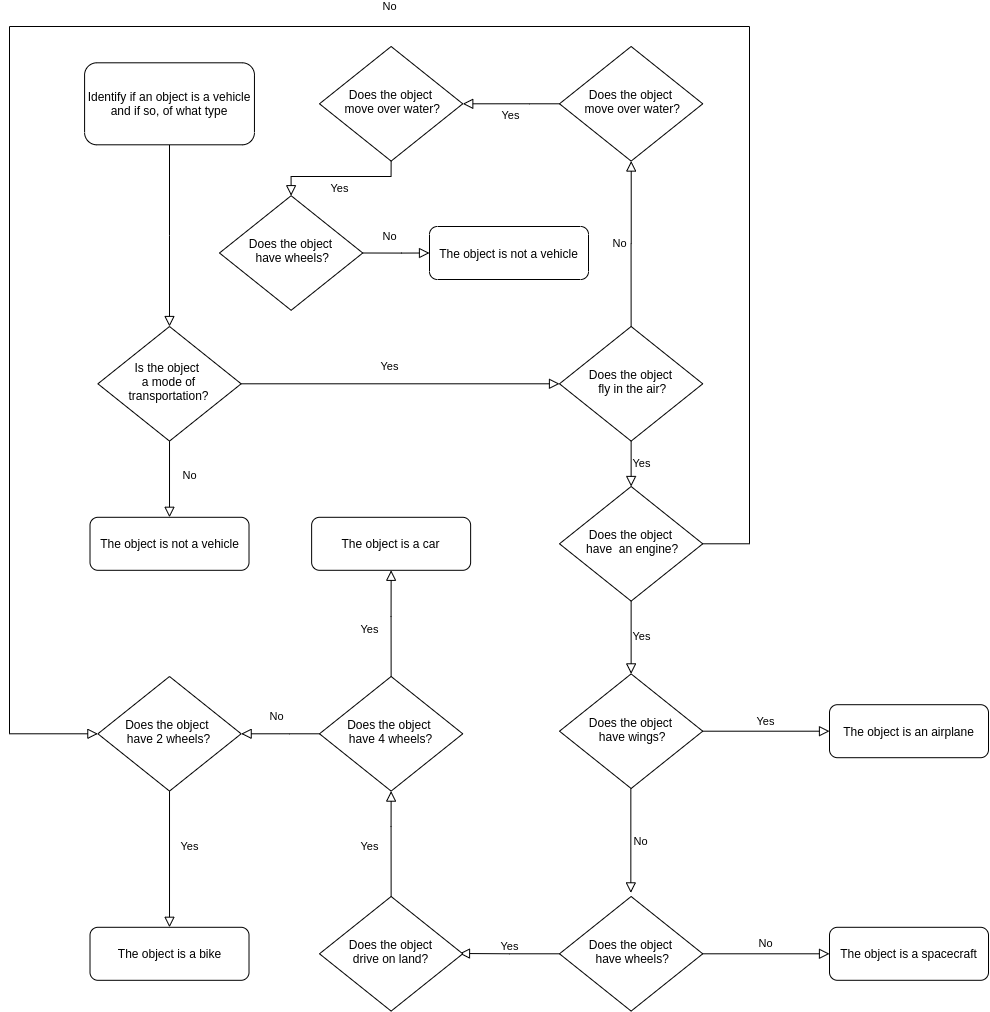
\includegraphics[width=\linewidth]{images/flowchart-prolog-vehicle-expert-system.png}
  \caption{This figure displays a decision tree that shows how our system could
  come to a conclusion in determining the type of a vehicle.}
  \label{fig:flowchart-expert-system}
\end{figure}


\section{Usage} \label{man-usage}
The application is run by providing the following command \textbf{isVehicle(X)}.
This will first check if we are looking to identify a vehicle.

If the user types `yes' the system agrees on a abstract data type `vehicle'.
This data type has multiple subtypes such as `land vehicle' or `air vehicle'.
At last we have the `unidentified vehicle'; this can be a car or boat.
The answer the system gives will be decided by the answers that the user provides.

\newpage
\section{Logic} \label{man-logic}
In this section we will provide an explanation of our code.
The code is included with comments to provide as reference for the explanation.

\begin{lstlisting}{}
% this will be the entry to our expert system
isVehicle(X) :- is_true('mode of transportation'), vehicle(X).

% the types of vehicle each type is part of an subtype
vehicle(airplane)  :- is_true('has wings'), air_vehicle().
vehicle(spaceCraft)  :- air_vehicle(), hasNoWheels().
vehicle(car)  :- is_true('has four wheels'), is_true('has engine'), land_vehicle() .
vehicle(motorBike) :- is_true('has two wheels'), land_vehicle().
vehicle(bicycle) :- is_true('no engine'), is_true('has two wheels'), land_vehicle().
vehicle(boat) :- is_true('has two wheels'), is_true('no engine'), boat_vehicle().

% the subtypes
land_vehicle() :-
	is_true('drives on land').
% check sub types
air_vehicle() :-
	is_true('flies in air'),
	is_true('has engine').

boat_vehicle() :-
	is_true("moves over water"),
    is_true("has no wheels").

hasNoWheels() :- not(is_true('has wheels')).

% helper method to generate questions
is_true(Q) :-
        format("~w?\n", [Q]),
        read(yes).
\end{lstlisting}

\begin{figure}[!h]
  \centering
  \includegraphics[height=7cm]{images/weirdfout.png}
  \caption{Rare foutmelding}
  \label{fig:rareFout}
\end{figure}{}

\newpage
\section{Queries} \label{man-queries}
Below will be listed several queries that each test a rule in our expert system.
The queries will be listed along with the responses of the system and comments
providing extra information.

\begin{lstlisting}{}
% Our expert system always starts with
% the question whether the object the
% the user is trying to identify is a
% vehicle by asking if the object is a "mode
% of transportation". If the user answers `no',
% the system knows the object is not a vehicle and
% will return `false' and stop guessing.
% If the user answers `yes', the system knows the
% object is a vehicle and will ask further questions
% to determine the specific type of vehicle. In the example
% below the user answers that "Chair" is not a mode of transportation
% so the system replies with false.
?- isVehicle(Chair).
mode of transportation?
|: no.

false.
\end{lstlisting}

\begin{lstlisting}{}
% In the query below we try to identify the object "JumboJet".
% after determining that the object is an actual vehicle, the
% system asks if the vehicle has wings. Because the user answers `yes'
% the system tries to match the object as an `air vehicle'. Being an
% air vehicle in our system consists of `flying in the air' and `having an
% engine'. Since the user answers yes to both of these questions, the system
% correctly asserts that the object is an airplane.
?- isVehicle(JumboJet).
mode of transportation?
|: yes.
has wings?
|: yes.
flies in air?
|: yes.
has engine?
|: yes.

JumboJet = airplane .
\end{lstlisting}

\begin{lstlisting}{}
% In the example below we try to identify `Sputnik1' as
% a spacecraft. A spacecraft in our system has the characteristics
% the earlier mentioned `air vehicle', but in addition has no wheels.
?- isVehicle(Sputnik1).
mode of transportation?
|: yes.
has wings?
|: no.
flies in air?
|: yes.
has engine?
|: yes.
has wheels?
|: no.

Sputnik1 = spaceCraft .
\end{lstlisting}

\begin{lstlisting}{}
% In the example below we try to identify a `Ferrari`.
% When the user says `no' to the questions about having wings and
% flying in the air, the system rules out the possibility of
% the object being any type of air vehicle like an airplane or spacecraft.
% Then our system asks if the object has four wheels. When the user says `yes',
% it tries to check if the object has an engine. If this is also true, the system
% tries to check if the object is a land vehicle by asking if the object drives on
% land. If this is true the object, Ferrari, is identified as a car.
?- isVehicle(Ferrari).
mode of transportation?
|: yes.
has wings?
|: no.
flies in air?
|: no.
has four wheels?
|: yes.
has enginge?
|: yes.
drives on land?
|: yes.

Ferrari = car .
\end{lstlisting}

\begin{lstlisting}{}
% In the example below the system ruled out
% that the object in question is not an air vehicle
% in the same way we have seen in the last example.
% Now however the user has answered `no' to the question
% whether the object has four wheels. The system tries
% to check if the object has two wheels. When the user answers
% `yes' to this question, it finally tries to check if the object
% drives on land to see if the object is land vehicle. The user
% gives the answer `yes' and the system identifies the object
% as a motorbike. This is one of the two, two-wheeled land vehicle types
% in our expert system. We will see the second type in this category in
% the next example.
?- isVehicle(Yamaha).
mode of transportation?
|: yes.
has wings?
|: no.
flies in the air?
|: no.
has four wheels?
|: no.
has two wheels?
|: yes.
drives on land?
|: yes.

Yamaha = motorBike .
\end{lstlisting}

\begin{lstlisting}{}
% In the example below we see the system thinks Gazelle is of type motorbike,
% because the user has not yet specified whether the object
% has an engine or not. In the online SWISH prolog interface
% there is the possibility to click next. When the user does this
% our system asks if the object doesn't have an engine. If the user
% replies `yes' our system correctly deduces that `Gazelle' is in
% fact not a motorbike, but a bicycle.
?- isVehicle(Gazelle).
mode of transportation?
|: yes.
has wings?
|: no.
flies in the air?
|: no.
has four wheels?
|: no.
has two wheels?
|: yes.
drives on land?
|: yes.

Gazelle = motorBike .
\end{lstlisting}
